\section{The vertical $\sigma$-coordinate}
\label{Scoord}

Following Song and Haidvogel \cite{Song94} but modified by
Shchepetkin and McWilliams \cite{SS2005}, the vertical coordinate has
been chosen to be:
\begin{equation}
   z = \zeta ( 1+\sigma) + h_c \sigma + (h - h_c) C(\sigma),
   \qquad \qquad -1 \leq \sigma \leq 0
\label{zetaa}
\end{equation}
where $h_c$ is either the minimum depth or a shallower depth above
which we wish to have more resolution.  $C(\sigma)$ is defined as:
\begin{equation}
   C(\sigma) = (1 - b) {\sinh (\theta \sigma) \over \sinh \theta } +
   b { \tanh [\theta ( \sigma + {1\over 2})] -
   \tanh ( {1\over 2} \theta) \over 
   2 \tanh ( {1\over 2} \theta) }
\end{equation}
where $\theta$ and $b$ are surface and bottom control parameters.
Their ranges are $0 < \theta \leq 20$ and $0 \leq b \leq 1$,
respectively.  Equation (\ref{zetaa}) leads to $z = \zeta$ for
$\sigma = 0$ and $z = h$ for $\sigma = -1$.

Some features of this coordinate system:
\begin{itemize}
   \item It is a generalization of the traditional $\sigma$-coordinate
   system.  Letting $\theta$ go to zero and using L'Hopital's rule,
   we get:
   \begin{equation}
      z = (\zeta + h)(1 + \sigma) - h
   \end{equation}
   which is the classic $\sigma$-coordinate.
   \item It is infinitely differentiable in $\sigma$.
   \item The larger the value of $\theta$, the more resolution is kept
   above $h_c$.
   \item For $b = 0$, the resolution all goes to the surface as
   $\theta$ is increased.
   \item For $b = 1$, the resolution goes to both the surface and the
   bottom equally as $\theta$ is increased.
   \item Some problems turn out to be sensitive to the value of
   $\theta$ used.
\end{itemize}
Figure \ref{fscd} shows the $\sigma$-surfaces for several values of $\theta$
and $b$ for one of our domains.  It was produced by a Matlab tool
written by Hernan Arango which is available from our web site (see
\S\ref{Ftp}).

\begin{figure}
\setlength{\unitlength}{10mm}
\begin{picture}(0,18)(0,0)
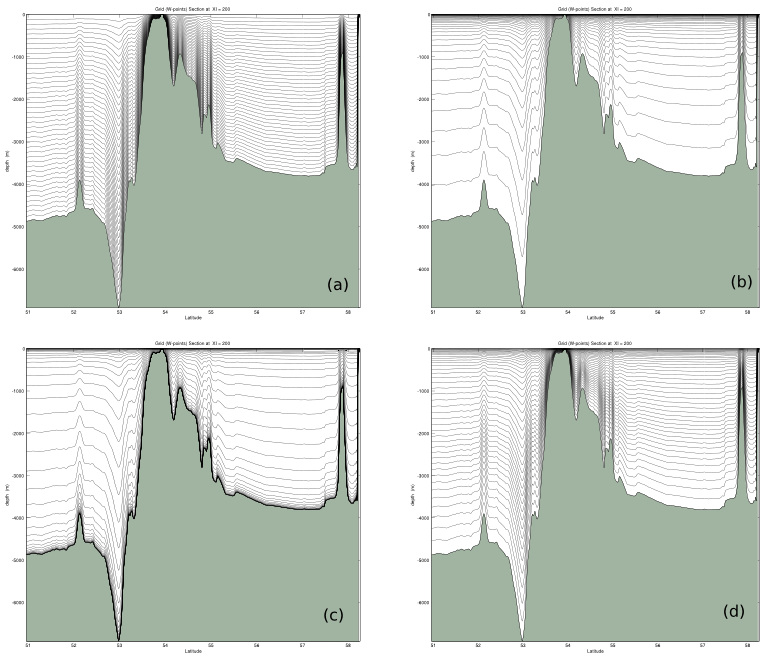
\includegraphics{pics/scoord}
\end{picture}

\caption{The $\sigma$-surfaces for the North Atlantic with (a) $\theta =
0.0001$ and $b = 0$, (b) $\theta = 8$ and $b = 0$, (c) $\theta = 8$
and $b = 1$.  (d) The actual values used in this domain were
$\theta = 5$ and $b = 0.4$.}
\label{fscd}
\end{figure}

We find it convenient to define:
\begin{equation}
   H_z \equiv {\partial z \over \partial \sigma} = (\zeta + h) +
   (h - h_c) {\partial C(\sigma) \over \partial \sigma} .
\end{equation}
The derivative of $C(\sigma)$ can be computed analytically:
\begin{equation}
   {\partial C(\sigma) \over \partial \sigma} = (1-b) {\cosh (\theta
   \sigma) \over
   \sinh \theta} \theta + b {\coth ( {1 \over 2} \theta) \over
   2 \cosh^2 [ \theta (\sigma + {1\over 2})] } \theta .
\end{equation}
However, we choose to compute $H_z$ discretely as $\Delta z/ \Delta
\sigma$ since this leads to the vertical sum of $H_z$ being exactly the
total water depth $D$.

Note that though we have used this form of $\sigma$-coordinate, ROMS
is written in such a way as to work with a variety of vertical
mappings. There is one feature which is critical, however. If the free
surface is at rest, $\zeta = 0$, you get one solution for the level
depths $z^{(0)}(k)$. In the case of nonzero $\zeta$, the
displacements must be proportional to $\zeta$ and to the original
distance from the bottom:
\begin{equation}
   z(k) =  z^{(0)} (k) + \zeta \left( 1 + {z^{(0)} (k) \over h}
   \right)
\end{equation}
or
\begin{equation}
   \Delta z(k) = \Delta z^{(0)} (k) \left( 1 + {\zeta \over h}
   \right)
\end{equation}
This ensures that the vertical mass fluxes generated by a purely
barotropic motion will vanish at every interface.
